\documentclass[12pt, a4 paper]{article}
% Set target color model to RGB
\usepackage[inner=2.0cm,outer=2.0cm,top=2.5cm,bottom=2.5cm]{geometry}
\usepackage{setspace}
\usepackage[rgb]{xcolor}
\usepackage{environ}
\usepackage{verbatim}
\usepackage{subcaption}
\usepackage{outlines}
\usepackage{enumitem}
\usepackage{amsgen,amsmath,amstext,amsbsy,amsopn,tikz,amssymb,tkz-linknodes}
\usepackage{fancyhdr}
\usepackage{pgfplots}
\usepackage{mathtools}
\usepackage[colorlinks=true, urlcolor=blue,  linkcolor=blue, citecolor=blue]{hyperref}
\usepackage[colorinlistoftodos]{todonotes}
\usepackage{rotating}

\linespread{1.6} % Double Line Spacing
\usetikzlibrary{arrows.meta,intersections,calc}

\hypersetup{%
pdfauthor={Vignesh Ravibaskar},%
pdfcreator={PDFLaTeX},%
pdfproducer={PDFLaTeX},%
}

% Our custom enumerate labelling, just making the outlines bold basically
\setlist[enumerate,1]{label=\textbf{\arabic*}}
\setlist[enumerate,2]{label=\textbf{({\alph*})}}
\setlist[enumerate,3]{label=\textbf{({\roman*})}}

\title{Differentiation}
\author{Derek, Vignesh}
\date{2020}

\newcommand{\comm}[1]{}
\NewEnviron{answer}{\vspace{3mm} \\ \color{blue} {\BODY} \color{black}}
%\NewEnviron{answer}{\color{blue} \comm{\BODY} \color{black}} % Use this method to hide all answers

\begin{document}

\maketitle

\textbf{DIFFERENTIATION [TBC Marks]}
\begin{outline}[enumerate]

 \1 Differentiate with respect to $x$ the following: %Question 1

 \2 $\ln (\ln ({x^2}))$\hfill[2]
 \begin{answer}
  Recall that $\frac{\mathrm{d}}{\mathrm{d}x}\ln(x^2)=\frac{2}{x}$
  \begin{align*}
   \frac{\mathrm{d}}{\mathrm{d}x}\ln (\ln ({x^2})) = \frac{2}{x\ln ({x^2})}
  \end{align*}
 \end{answer}

 \2 $4^{\cos 4x}$\hfill[2]
 \begin{answer}
  Recall that you can express $4^{\cos4x}$ as $\mathrm{e}^{\ln4cos4x}$
  \begin{align*}
   \frac{\mathrm{d}}{\mathrm{d}x}4^{\cos 4x} & =\frac{\mathrm{d}}{\mathrm{d}x}\mathrm{e}^{\ln4cos4x} \\
                                             & = -8\ln2 \cdot \sin4x \cdot \mathrm{e}^{\ln4cos4x}    \\
                                             & = -8\ln2 \cdot \sin4x \cdot 4^{\cos4x}
  \end{align*}
 \end{answer}

 \2 $\tan ^{ - 1}(xy)$\hfill[2]
 \begin{answer}
  Recall that differentiating $xy$ wrt $x$ gives you $y+x\frac{\mathrm{d}y}{\mathrm{d}x}$
  \begin{align*}
   \frac{\mathrm{d}}{\mathrm{d}x}\tan ^{ - 1}(xy) & = \frac{y+x\frac{\mathrm{d}y}{\mathrm{d}x}}{1+(xy)^2}
  \end{align*}
 \end{answer}

 \2 $\dfrac{{{x^2}}}{3} - \dfrac{{{y^2}}}{4} = 1$\hfill[2]
 \begin{answer}
  \begin{align*}
   \frac{\mathrm{d}}{\mathrm{d}x}\left[\dfrac{{{x^2}}}{3} - \dfrac{{{y^2}}}{4}\right] = \frac{2}{3}x-\frac{1}{2}y\cdot\frac{\mathrm{d}y}{\mathrm{d}x} = 0
  \end{align*}
 \end{answer}

 \1 Solve the following differential equations: %Question 2
 \begin{answer}
  For this section, we will collect similar terms ($\mathrm{d}y, y$) terms on the same side before integrating them respectively
 \end{answer}

 \2 $\dfrac{{{\rm{d}}y}}{{{\rm{d}}x}} = 2y,\;y = 1{\textrm{ when }}\,x = 1$ \hfill[2]
 \begin{answer}
  \begin{align*}
   \frac{\mathrm{d}y}{y} & = 2\mathrm{d}x                     \\
   \ln|y|                & = 2x+C \implies C=\ln(1)-2(1) = -2 \\
   y                     & = \mathrm{e}^{2x-2}
  \end{align*}
 \end{answer}

 \2 $\dfrac{{{\rm{d}}x}}{{{\rm{d}}t}} = 4({x^2} + x + 1)$ \hfill[3]
 \begin{answer}
  \begin{align*}
   \frac{\mathrm{d}x}{x^2+x+1}                                & = 4\mathrm{d}t \\
   \frac{\mathrm{d}x}{(x+\frac{1}{2})^2+(\frac{\sqrt3}{2})^2} & = 4\mathrm{d}t \\
   \frac{2}{\sqrt3}\tan^{-1}\left(\frac{2x+1}{\sqrt3}\right)  & = 4t + C       \\
   x = \frac{1}{2}\left[\sqrt3\tan\left(\frac{8\sqrt3}{3}t + C\right)-1\right]
  \end{align*}
 \end{answer}

 \2 $\dfrac{{{\rm{d}}y}}{{{\rm{d}}x}} = \dfrac{{ - {\mathrm{e}^{ - 3x}}}}{{3y}}$ \hfill[3]
 \begin{answer}
  \begin{align*}
   y\,\mathrm{d}y & = -\frac{\mathrm{e}^{-3x}}{3} \mathrm{d}x \\
   \frac{1}{2}y^2 & = \frac{1}{9}\mathrm{e}^{-3x} + C         \\
   y              & = \sqrt{\frac{2}{9}\mathrm{e}^{-3x} + C}
  \end{align*}
 \end{answer}

 \1 The parametric equations of curve C are: \[x = t + 1,\;y = \frac{1}{{{t^2} + 2t + 2}}{\textrm{ where }} - 3 \leq t \leq 1.\] %Question 3

 \2 Find the Cartesian equation of $C$. \hfill[2]
 \begin{answer}
  Notice that $t^2+2t+2 = (t+1)^2 = x^2\implies$ The Cartesian equation is $y=\frac{1}{x^2}$
 \end{answer}

 \2 Find the equation of the tangent to the curve $C$ when $t=2$.\hfill[3]
 \begin{answer}
  Recall that for a parametric equation, $\frac{\mathrm{d}y}{\mathrm{d}x}=\frac{\mathrm{d}y}{\mathrm{d}t}\div\frac{\mathrm{d}x}{\mathrm{d}t}$. However, it is much simpler to find $\frac{\mathrm{d}y}{\mathrm{d}x}$ directly
  \begin{align*}
   \frac{\mathrm{d}y}{\mathrm{d}x}                    & = -\frac{2}{x^3}             \\
   \left.\frac{\mathrm{d}y}{\mathrm{d}x}\right|_{t=2} & = -\frac{2}{2+1}             \\
                                                      & = -\frac{2}{3}               \\\\
   y-y|_{t=2}                                         & = -\frac{2}{3}(x-3)          \\
   y - \frac{1}{9}                                    & = -\frac{2}{3}(x-3)          \\
   \implies y                                         & = -\frac{2}{3}x+2\frac{1}{9}
  \end{align*}
 \end{answer}

 \1 Two variables $x$ and $y$ vary with time $t$ in minutes and are connected by the equation $\sin (xy) = \frac{1}{2}$. Given that $x$ increases at a rate of 3 units per minute, find the (maximum possible) rate of decrease of $y$ when $y = 1$. \hfill[4] %Question 4
 \begin{answer}
  Recall that differentiating $xy$ wrt $x$ gives you $y+x\frac{\mathrm{d}y}{\mathrm{d}x}$. Therefore, we will first differentiate $\sin (xy) = \frac{1}{2}$ wrt $x$.
  \begin{align*}
   \frac{\mathrm{d}}{\mathrm{d}x}\sin (xy)  & = \left(y+x\frac{\mathrm{d}y}{\mathrm{d}x}\right)\cos(xy) = 0           \\
   \implies \frac{\mathrm{d}y}{\mathrm{d}x} & = -\frac{y}{x}                                                          \\\\
   \frac{\mathrm{d}y}{\mathrm{d}t}          & = \frac{\mathrm{d}y}{\mathrm{d}x} \cdot \frac{\mathrm{d}x}{\mathrm{d}t} \\
                                            & = -\frac{3y}{x}                                                         \\
  \end{align*}
  To get the maximum rate of decrease, we find the minimum value of $x$
  \begin{align*}
   x|_{y=1}                                                                      & = \arcsin\left(\frac{1}{2}\right)\div 1 = \frac{\pi}{6} + 2k\pi \quad\textrm{OR}\quad \frac{5\pi}{6} + 2k\pi, k\in\mathbb{Z} \\
   \left.\frac{\mathrm{d}y}{\mathrm{d}t}\right|_{x=\frac{\pi}{6}, y=\frac{1}{2}} & = -\frac{9}{\pi}
  \end{align*}
  The maximum rate of decrease is $\frac{9}{\pi}$ units per minute.
 \end{answer}

 \1 The parametric equations of curve C are: \[x = 1 + {\mathrm{e}^{ - at}},\;y = {\mathrm{e}^{at}} + {\mathrm{e}^{ - at}}\;{\textrm{ where }}t \geq 0.\] %Question 5

 \2  Sketch $C$, including all stationary points and asymptotes where applicable.\hfill[2]
 \begin{answer}
  \color{black}
  \begin{tikzpicture}
   \begin{axis}[
     axis lines = center,
     xlabel = $x$,
     ylabel = $y$,
     xmin = 0, xmax = 2,
     ymin = 0, ymax = 10,
     legend pos=outer north east
    ]
    \addplot [
     domain=0:5,
     samples=100,
     color=blue,
    ]
    ({1+e^(-x)},
    {e^x-e^(-x)});
    \addlegendentry{$(1 + {\mathrm{e}^{ - at}}, {\mathrm{e}^{at}} + {\mathrm{e}^{ - at}})$}

    \addplot[black, mark=*, only marks] coordinates {(1,0)};
    \node[label={180:{$x=1$}}] at (axis cs:1,2) {};
    \addplot[mark=none, black, ultra thick,dotted] coordinates {(1,0) (1,12)};

    \addplot[black, mark=*, only marks] coordinates {(0,0)};
    \node[label={0:{$y=0$}}] at (axis cs:0.5,0.5) {};
   \end{axis}
  \end{tikzpicture}

 \end{answer}

 \2 Find the equation of the normal to the curve $C$ at $t = \frac{\ln{2}}{{2a}}$.\hfill[3]
 \begin{answer}
  Recall that for a parametric equation, $\frac{\mathrm{d}y}{\mathrm{d}x}=\frac{\mathrm{d}y}{\mathrm{d}t}\div\frac{\mathrm{d}x}{\mathrm{d}t}$. Furthermore, the gradient of the normal at a given point is equal to $-[\frac{\mathrm{d}y}{\mathrm{d}x}]^{-1}$ at that point
  \begin{align*}
   \frac{\mathrm{d}y}{\mathrm{d}x}=\frac{a\mathrm{e}^{at}-a\mathrm{e}^{-at}}{-a\mathrm{e}^{-at}} = 1-\mathrm{e}^{2at}
  \end{align*}
  We will now find the values for $\frac{\mathrm{d}y}{\mathrm{d}x}, x, y$ when $t=\frac{\ln2}{2a}$ to get the equation of the normal
  \begin{align*}
   \left.\frac{\mathrm{d}y}{\mathrm{d}x}\right|_{t=2}     & = -1                                      \\
   (x,y)|_{t=2}                                           & = (1+\frac{\sqrt2}{2}, \frac{3\sqrt2}{2}) \\
   \implies \textrm{Eqn Normal:}\quad y-\frac{3\sqrt2}{2} & = (x-1-\frac{\sqrt2}{2})                  \\
   y                                                      & = x-1+\sqrt2
  \end{align*}
 \end{answer}

 \2 What can be said about the normals to the curve $C$ as $t$ gets large?\hfill[1]
 \begin{answer}
  As $t\rightarrow\infty$, $\mathrm{e^{2at}}\rightarrow\infty$, thus, $-[\frac{\mathrm{d}y}{\mathrm{d}x}]^{-1} = -\frac{1}{1-\mathrm{e}^{2at}}\rightarrow0\implies$ the normals become parallel to the $x$-axis
 \end{answer}


 \1 A boy throws a rock in the air. It is launched at an angle $\theta$ to the horizontal ground, where $0 < \theta  < \frac{\pi }{2}$. As shown in the diagram, its position in the air $(x,y)$, where $x$ is the horizontal position and $y$ is the vertical position, is approximated by: \[x = (20\cos \theta )t,\,\;y = (20\sin \theta )t - 5{t^2},\]where $t$ is the time in seconds.
 \[
  \begin{tikzpicture}
   \begin{axis}[
     axis lines = center,
     xlabel = $x$,
     ylabel = $y$,
     xmin = 0, xmax=4.5,
     ymin = 0, ymax=4.5,
     xticklabels = {,,},
     yticklabels = {,,},
     legend pos=north east
    ]
    \addplot [
     domain=0:3,
     samples=100,
     color=blue,
    ]
    {x-0.2*x^2};
    \node[label] at (axis cs:0.5,0.23) {$\theta$};
    \addlegendentry{Path of stone};
   \end{axis}
   \draw[->,very thick] (0,0) -- (2,2);
   \draw[thick] (0:0.5) arc (0.5:45:0.5);
  \end{tikzpicture}
 \]

 \2 Find, in terms of $\theta$,

 \3 The time taken for the toy plane to hit the ground;\hfill[2]
 \begin{answer}
  When the toy plane hits the ground, $y=0$
  \begin{align*}
   (20\sin \theta )t - 5{t^2} = -5t(t-4\sin\theta) & = 0                                   \\
   \implies t                                      & = 0 \quad\textrm{OR}\quad 4\sin\theta
  \end{align*}
  It takes $(4\sin\theta)$s for the toy plane to hit the ground
 \end{answer}

 \3 The maximum height reached by the toy plane;\hfill[2]
 \begin{answer}
  Note that $y(t)$ is symmetrical about the centre $t=2\sin\theta$ and thus, it is at the maximum at this time.
  \begin{align*}
   y|_{t=2\sin\theta} = (20\sin\theta)\cdot2\sin\theta - 5(2\sin\theta)^2 = 20\sin^2\theta
  \end{align*}
  The maximum height is $(20\sin^2\theta)$ units.
 \end{answer}

 \3 The horizontal distance travelled by the toy plane.\hfill[2]
 \begin{answer}
  The horizontal distance is equal to the $x$ value when $t=4\sin\theta$ as we found in \textbf{(a)(i)}
  \begin{align*}
   x|_{t=4\sin\theta} = (20\cos\theta)\cdot4\sin\theta = 40\sin2\theta
  \end{align*}
  The maximum horizontal distance is $(40\sin2\theta)$ units.
 \end{answer}

 \2 Find the angle $\theta$ at which the toy plane should be thrown to attain the maximum horizontal distance.\hfill[2]
 \begin{answer}
  Intuitively, we assume that $\theta=45^\circ$ but let us verify this.
  \begin{align*}
   \frac{\mathrm{d}x}{\mathrm{d}\theta}     & = 80\cos2\theta   \\
   \frac{\mathrm{d}^2x}{\mathrm{d}\theta^2} & = -160\sin2\theta \\
  \end{align*}
  When $\frac{\mathrm{d}x}{\mathrm{d}\theta}=0$, $\theta=45^\circ$ and $\frac{\mathrm{d}^2x}{\mathrm{d}\theta^2}=-160<0\implies x$ is at a maximum
 \end{answer}

 \1 A hopper in a butter processing factory is used to store pre-processed butter before it is discharged to the next stage of the manufacturing process. One such hopper is designed with the dimensions as follows: %Question 7
 \[
  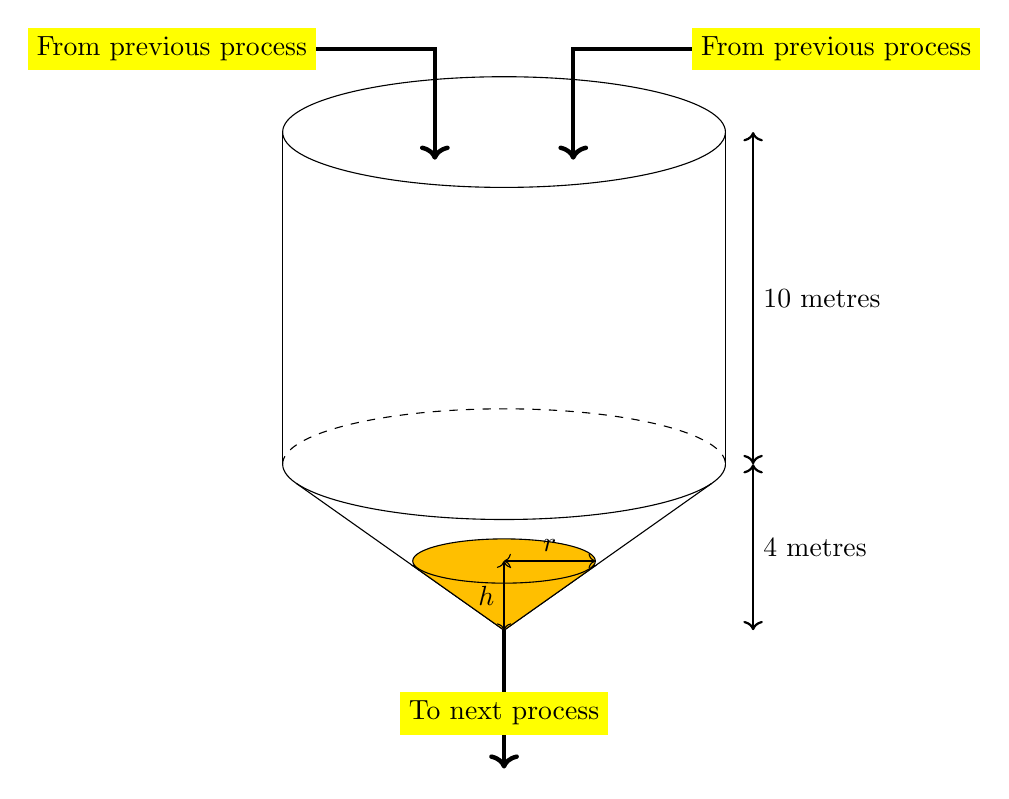
\begin{tikzpicture}
   \draw (0,0) ellipse (80pt and 20pt); %Begin Cylinder
   \draw (-80pt,0) -- (-80pt,-120pt);
   \draw (80pt,0) -- (80pt,-120pt);
   \draw (-80pt,0) -- (-80pt,-120pt);
   \draw[dashed] (-80pt,-120pt) arc (180:0:80pt and 20pt);
   \draw (-80pt,-120pt) arc (180:360:80pt and 20pt);
   \draw[<->,thick] (90pt,0) -- (90pt,-60pt) node[right] {10 metres} -- (90pt,-120pt);%End Cylinder
   \draw (-75pt,-127pt) -- (0, -180pt); %Begin Cone
   \draw (0,-180pt) -- (75pt,-127pt);
   \draw[<->,thick] (90pt,-120pt) -- (90pt,-150pt) node[right] {4 metres} -- (90pt,-180pt);%End Cone
   \draw[->,ultra thick] (-120pt,30pt) node [fill=yellow]{From previous process}-- (-25pt,30pt) -- (-25pt,-10pt); %Begin Butter Line
   \draw[->,ultra thick] (120pt,30pt) node [fill=yellow]{From previous process}-- (25pt,30pt) -- (25pt,-10pt);
   \draw[->,ultra thick] (0,-180pt) -- (0,-210pt) node[fill=yellow]{To next process} -- (0,-230pt); %End Butter Line
   \filldraw [orange!50!yellow,draw=black](0,-180pt) -- (33pt,-156.68pt) -- (-33pt,-156.68pt) -- cycle; %Begin Filled Butter
   \filldraw [orange!50!yellow,draw=black](0,-155pt) ellipse (33pt and 8pt);
   \draw[<->] (0,-155pt) -- (16.5pt, -155pt) node [above]{$r$}-- (33pt,-155pt);
   \draw[<->] (0,-155pt) -- (0, -167.5pt) node [left]{$h$}-- (0,-180pt); %End Filled Butter
  \end{tikzpicture}
 \]
 The hopper can be said to be a cylinder attached to a cone, both of radius 3 metres. At $t$ hours, the height of the butter in the cone is $h$ and the radius of the liquid surface is $r$. At time $t = 0$ hours, the depth of butter is 3 metres.\\

 If the butter is allowed to flow out of the cone at $- 3\textrm{ m}^3{\textrm{ per hour}}$,
 \2 Show that ${h^2}\dfrac{{{\mathrm{d}}h}}{{{\mathrm{d}}t}} =  - \dfrac{{16}}{{3\pi }}$.\hfill[3]

 \2 Calculate the exact time it takes for the butter to completely drain out.\hfill[3]

 \2 Ignore the changes in \textbf{(a)} i.e. currently, $t = 0$ and $h = 3$. An operator wants to fill up the entire hopper with butter within 48 hours, with a net inflow of $k\textrm{ m}^3{\textrm{ per hour}}$. Find $k$.\hfill[4]

 \1 A scientist set up an experiment as shown below:
\[
 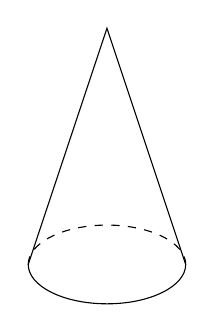
\begin{tikzpicture}
    \draw (-1,0) arc (180:360:1cm and 0.5cm) -- (0,3) -- cycle;
    \draw[dashed] (-1,0) arc (180:0:1cm and 0.5cm);
\end{tikzpicture}
\]

 \1 An inflatable cube is inscribed inside an inflatable sphere such that the cross-section of the figure is as shown:
 \[
 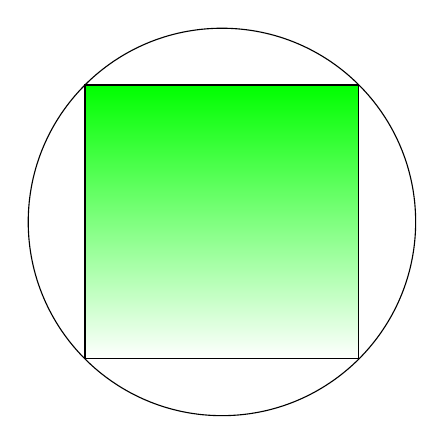
\begin{tikzpicture}
   \draw (0,0) circle (70pt);
   \shade[top color=green,bottom color=white,draw=black] (49.497475pt,-49.497475pt) rectangle (-49.497475pt,49.497475pt);
 \end{tikzpicture}
   \]
  The cube has sides of length 1 unit initially. When the cube is allowed to inflate, the length of its side increase at a rate of $3t$, where $t$ is the time in minutes. As the cube expands, the sphere expands uniformly and bursts when it has a volume of $27\pi$ units$^3$.

  \2 Express the length of one of the cube's sides $s$ as a function of time $t$. \hfill[2]

  \2 Calculate the time taken for the sphere to burst. \hfill[3]

 \1 In a city of Martians, the birth and death rates are high. The population is $x$ Martians (in thousands) and $t$ is the time in years since 2300. The birth rate is 2 times the population per year and the death rate at 1.5 times the square of the population per year.

 \2 Show that $\dfrac{{{\textrm{d}}x}}{{{\textrm{d}}t}} = \dfrac{1}{2}(4x - 3{x^2})$\hfill[2]
 \2 Express $\dfrac{1}{{x(4 - 3x)}}$ as a sum of partial fractions.\hfill[2]
 \2 Given that, in year 2300, the population was 1000, solve the differential equation in \textbf{(a)}.\hfill[4]



\end{outline}

\end{document}
